\subsection{Intelligence Artificielle et NPC}

Pour rendre notre jeu plus vivant et permettre aux joueurs de se mêler à la foule,
il nous fallait créer des IA se déplaçant dans la ville.
Pour cela, nous avons décider d'utiliser des NavMesh pour créer des zones où les 
NPC peuvent se balader d'un point à un autre.
Pour ne pas rendre leur comportement linéaire et trop prévisible, ce qui gâcherait inéluctablement le jeu,
ils se déplacent de manière aléatoire  vers un point quelconque défini dans une liste de coordonnées.
Les NPC ont donc des comportements pseudo-aléatoires (même s'ils empruntent toujours le chemin le plus court entre deux objectifs) qui permettent
aux joueurs de se fondre plus facilement dans la masse. En d'autres termes, en faisait se comporter les IA comme des joueurs, on évite aux joueurs
d'avoir à se comporter comme des robots.\\

L’outil de navigation est assez poussé, et permet de définir les dimensions des personnages,
ainsi que la hauteur de laquelle ils peuvent sauter et les pentes qu’ils peuvent emprunter.
Ici, la pente maximale est de 33.4°, mais si ce chiffre avait été plus élevé,
les pentes seraient devenues praticables (bleues)\footnote{Voir fugure 3}, et les personnages auraient pu
monter sans utiliser les escaliers (ce qui n’est évidemment pas le but).


Pour rendre ces IA plus humaines, les joueurs peuvent les bousculer et les étourdir en courant vers eux.
Ils reprenent leur trajet au bout de quelques secondes. Il faudra ainsi, dans les prochaines versions, 
améliorer la navigation afin que le chemin emprunté ne soit pas toujours le plus court. 
\newline

\begin{figure}[h!]
        \centering
        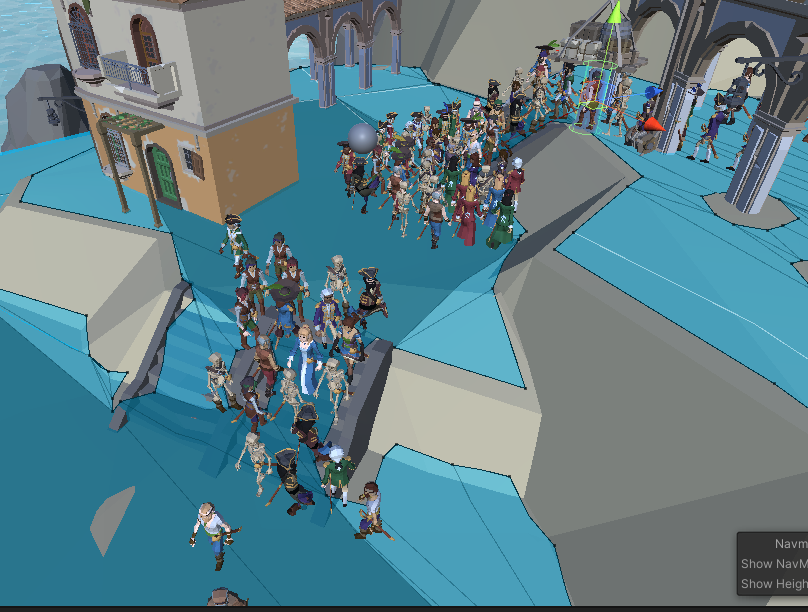
\includegraphics[scale=0.3]{ia_stairs_bug.png}
        \caption{Problème rencontré lorsque de nombreuses IA vont au même endroit}
\end{figure}